% A conference talk for "Sparse Attention for Long-Context Retrieval".
\documentclass[aspectratio=169]{beamer}
\usetheme{metropolis}
\usepackage{booktabs}
\usepackage{amsmath}

\newcommand{\R}{\mathbb{R}}

\title{Sparse Attention for Long-Context Retrieval}
\subtitle{Reading less of the context, losing none of the answer}
\author{Helena Marsh \and Tomás Okafor \and Ingrid Sæther}
\institute{Northfield University \quad Lighthouse Research Lab}
\date{ICLR Workshop on Long Context, April 2026}

\begin{document}

\begin{frame}
  \titlepage
\end{frame}

\begin{frame}{Outline}
  \tableofcontents
\end{frame}

\section{The problem}

\begin{frame}{Long contexts are mostly irrelevant}
  \begin{itemize}
    \item A 128k-token context holds a whole repository or a year of notes.
    \pause
    \item For any one question, a few passages carry most of the attention.
    \pause
    \item Dense attention still reads \alert{every} key, every layer.
  \end{itemize}
\end{frame}

\begin{frame}
  \frametitle{Where the time goes}
  \begin{columns}[T]
    \begin{column}{0.48\textwidth}
      \textbf{Decoding at 128k tokens}
      \begin{itemize}
        \item 71\% memory traffic for keys and values
        \item 18\% matrix multiplies
        \item 11\% everything else
      \end{itemize}
    \end{column}
    \begin{column}{0.48\textwidth}
      \begin{block}{Observation}
        Reading fewer keys is worth more than computing faster on the ones we read.
      \end{block}
    \end{column}
  \end{columns}
\end{frame}

\section{Sieve}

\begin{frame}{Scout, then read}
  Summarise each block of $b$ keys by its mean and spread:
  \[
    s_i(q) = q \cdot \bar{k}_i + \tfrac{1}{2}\,\lVert q \rVert\, \sigma_i
  \]
  Keep the top $k$ blocks, plus the local and global blocks:
  \begin{equation*}
    S_t = \operatorname{top}_k\bigl(s_1, \dots, s_B\bigr) \cup \{t\} \cup G
  \end{equation*}
  \begin{alertblock}{Guarantee}
    The output error is at most $2R\,\delta(S)$, twice the value norm times the discarded attention mass.
  \end{alertblock}
\end{frame}

\begin{frame}{What it selects}
  \begin{columns}[c]
    \begin{column}{0.55\textwidth}
      \centering
      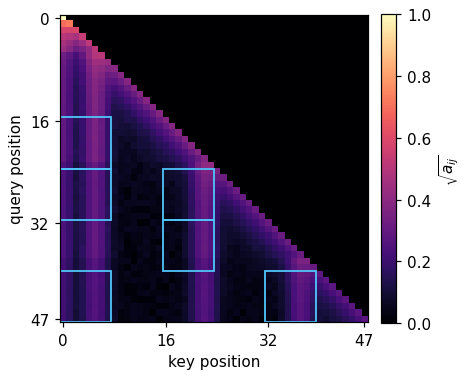
\includegraphics[width=\linewidth]{../paper/figures/attention.png}
    \end{column}
    \begin{column}{0.4\textwidth}
      \begin{exampleblock}{Layer 18, head 3}
        Outlined blocks are the ones \textsc{Sieve} reads. They cover the
        bright columns: the first token and three retrieved passages.
      \end{exampleblock}
    \end{column}
  \end{columns}
\end{frame}

\section{Results}

\begin{frame}{Accuracy at 128k tokens}
  \centering
  \begin{tabular}{lrrr}
    \toprule
    Method & Needle & Multi-doc QA & Keys read \\
    \midrule
    Dense & 99.1 & 71.4 & 131k \\
    BigBird & 88.3 & 63.0 & 12k \\
    \textsc{Sieve} ($k=16$) & \textbf{98.9} & \textbf{71.0} & 11k \\
    \bottomrule
  \end{tabular}
  \vspace{1em}

  Within 0.4 points of dense attention, with $11\times$ fewer keys.
\end{frame}

\begin{frame}{Takeaways}
  \begin{enumerate}
    \item Most keys don't matter, and block summaries find the ones that do.
    \item The error is bounded by the attention mass we skip.
    \item No retraining, no index, no second model.
  \end{enumerate}
\end{frame}

\begin{frame}[standout]
  Questions?

  \vspace{1em}
  \small\url{https://example.org/sieve}
\end{frame}

\end{document}
